%%%%%%%%%%%%%%%%%%%%%%%%%%%%%%%%%%%%%%%%%%%%%%%%%%%%%%%%%%%%%%%%%%%%%%%%%%%%%%%%
\section{Why Workflows}

%%%%%%%%%%%%%%%%%%%%%%%%%%%%%%%%%%%%%%%%%%%%%%%%%%%%%%%%%%%%%%%%%%%%%%%%%%%%%%%%
\begin{frame}
    \frametitle{Outline}
    \begin{columns}[t]
        \begin{column}{.5\textwidth}
            \tableofcontents[sections={1-7},currentsection]
        \end{column}
        \begin{column}{.5\textwidth}
            \tableofcontents[sections={8-15},currentsection]
        \end{column}
    \end{columns}
\end{frame}

%%%%%%%%%%%%%%%%%%%%%%%%%%%%%%%%%%%%%%%%%%%%%%%%%%%%%%%%%%%%%%%%%%%%%%%%%%%%%%%%
\begin{frame}
  \frametitle{What is this about?}
   \begin{question}[Questions]
   	 \begin{itemize}
        \item I can code everything! Can I?
        \item What is the benefit of a workflow system?
        \item What distinguishes a workflow system from a ``pipeline''?
     \end{itemize}
   \end{question}
   \begin{docs}[Objectives]
   	  \begin{enumerate}
         \item Introducing workflow engines (particularly \Snakemake)!
      \end{enumerate}
   \end{docs}
\end{frame}  

%%%%%%%%%%%%%%%%%%%%%%%%%%%%%%%%%%%%%%%%%%%%%%%%%%%%%%%%%%%%%%%%%%%%%%%%%%%%%%%%
\begin{frame}
  \frametitle{Data Analysis}
  \begin{onlyenv}<1| handout:0>
    \begin{tikzpicture}
      \path[use as bounding box] (0.7,0) rectangle (12,8);
      \node[inner sep=0pt] (analysis_1) at (5,6)
         {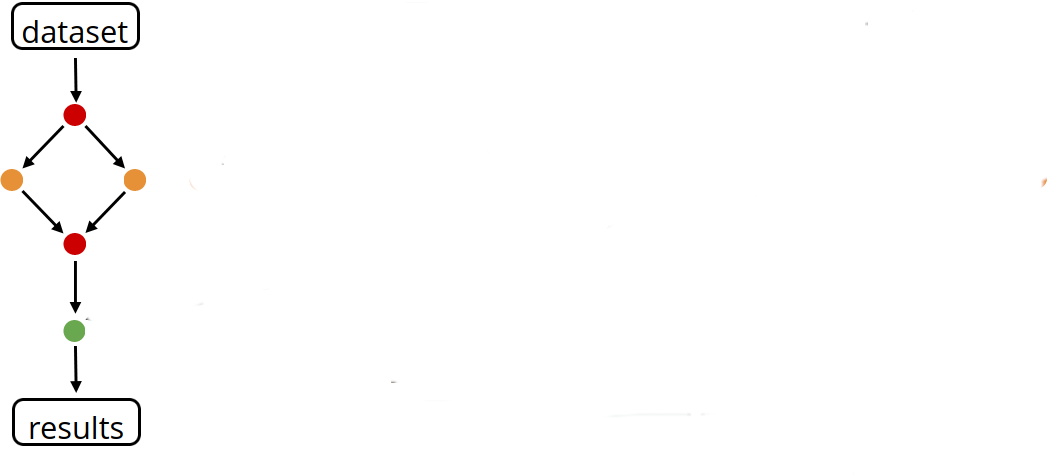
\includegraphics[width=0.7\textwidth]{Snakemake/analysis_1.png}};   
      \node at (7, 3.5) %[below=-0.4cm of analysis_1, xshift=2.7cm] at (current page.center)
         {
\includegraphics[width=0.45\textwidth]{Snakemake/phd_left.png}};
      \node at (6, 1) {\begin{minipage}{0.75\textwidth}\footnotesize
                        Idea from the official \lhref{https://slides.com/johanneskoester/snakemake-tutorial}{\Snakemake} course (with permission), image from \lhref{https://phdcomics.com/comics.php}{PhD comics}.
                       \end{minipage}
      };
    \end{tikzpicture}    
  \end{onlyenv}
  
  \begin{onlyenv}<2| handout:1>
    \begin{tikzpicture}
      \path[use as bounding box] (0.7,0) rectangle (12,8);
      \node[inner sep=0pt] (analysis_full) at (5,6)
         {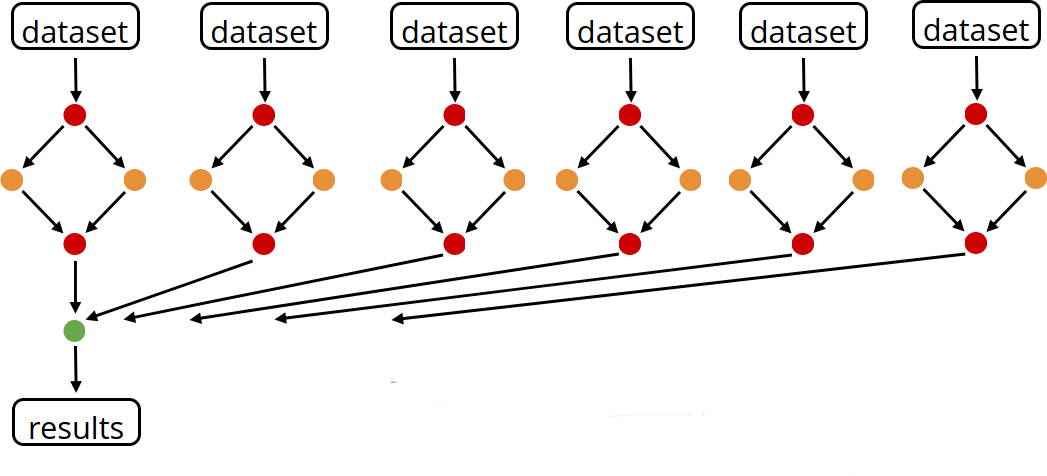
\includegraphics[width=0.7\textwidth]{Snakemake/analysis_full.png}};   
      \node at (7,3.5) % [below=-0.4cm of analysis_full, xshift=2.7cm]
         {
\includegraphics[width=0.45\textwidth]{Snakemake/phd_full.png}};
      \node at (6, 1) {\begin{minipage}{0.75\textwidth}\footnotesize
                        Idea from the official \lhref{https://slides.com/johanneskoester/snakemake-tutorial}{\Snakemake} course (with permission), image from \lhref{https://phdcomics.com/comics.php}{PhD comics}.
                       \end{minipage}
      };
    \end{tikzpicture}
  \end{onlyenv}
\end{frame}

%%%%%%%%%%%%%%%%%%%%%%%%%%%%%%%%%%%%%%%%%%%%%%%%%%%%%%%%%%%%%%%%%%%%%%%%%%%%%%%%
\begin{frame}
  \frametitle{Goals of Reproducibility}
  \Huge
  \begin{enumerate}
   \item Dispel Doubts
   \item Facilitate Further Experimentation
  \end{enumerate}
  \vfill
  \footnotesize{Idea from \lhref{https://elephly.net/downies/2023-dfn-slides.pdf}{DFN slides}.}
\end{frame}

%%%%%%%%%%%%%%%%%%%%%%%%%%%%%%%%%%%%%%%%%%%%%%%%%%%%%%%%%%%%%%%%%%%%%%%%%%%%%%%%
\begin{frame}
  \frametitle{Reproducible Data Analysis}
  \begin{onlyenv}<1| handout:0>
    \begin{tikzpicture}
      \path[use as bounding box] (0.7,0) rectangle (12,8);
      \node at (5.5, 5.5) {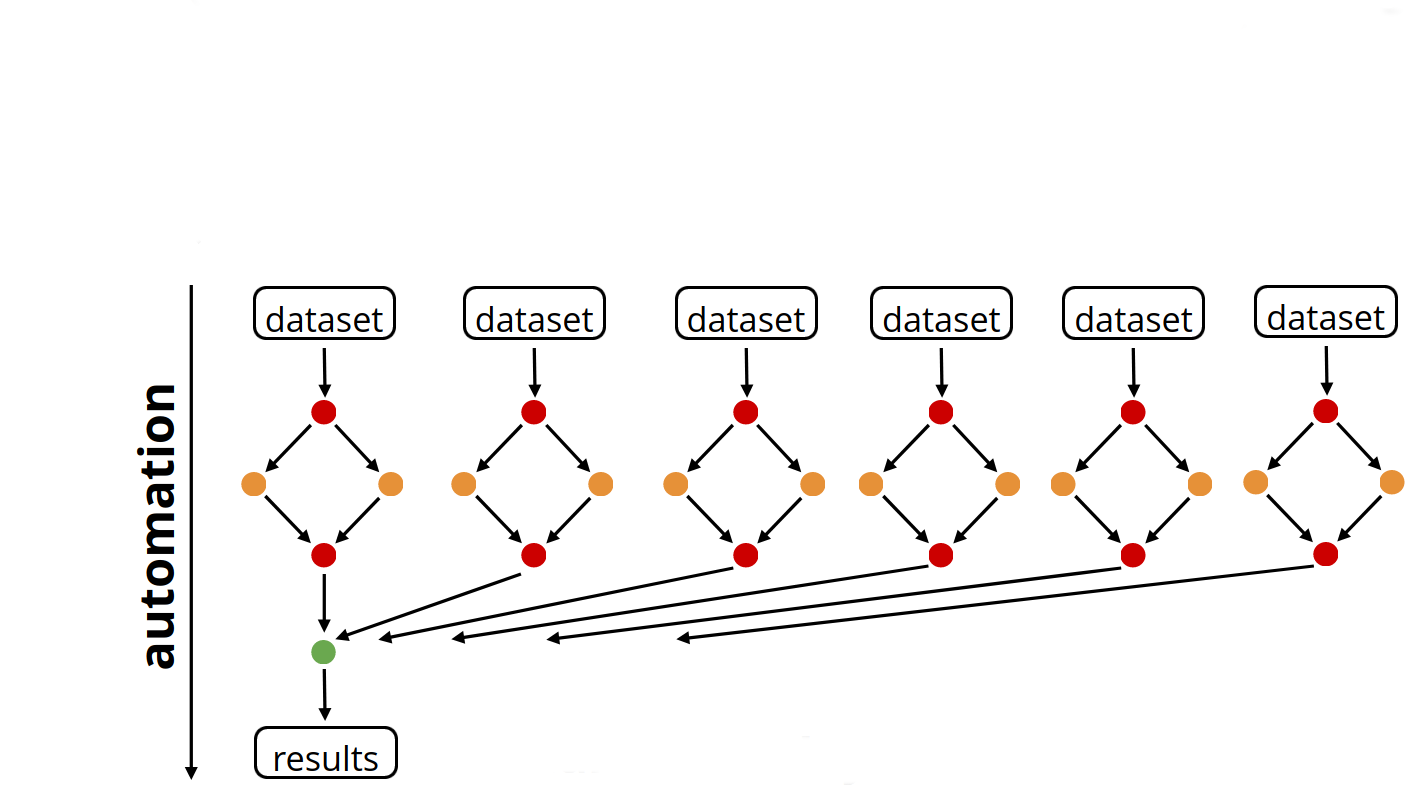
\includegraphics[width=0.7\textwidth]{Snakemake/automation.png}};
      \node at (8, 2.5) {\begin{minipage}{0.65\textwidth}
                             \textbf{From raw data to final figures:}
                             \begin{itemize}
                                \item \textbf{document} parameters, tools, versions
                                \item \textbf{execute} without manual intervention
                              \end{itemize}
                           \end{minipage}
                           };
    \end{tikzpicture}
  \end{onlyenv}
  \begin{onlyenv}<2| handout:0>
    \begin{tikzpicture}
      \path[use as bounding box] (0.7,0) rectangle (12,8);
      \node at (5.5, 5.5) {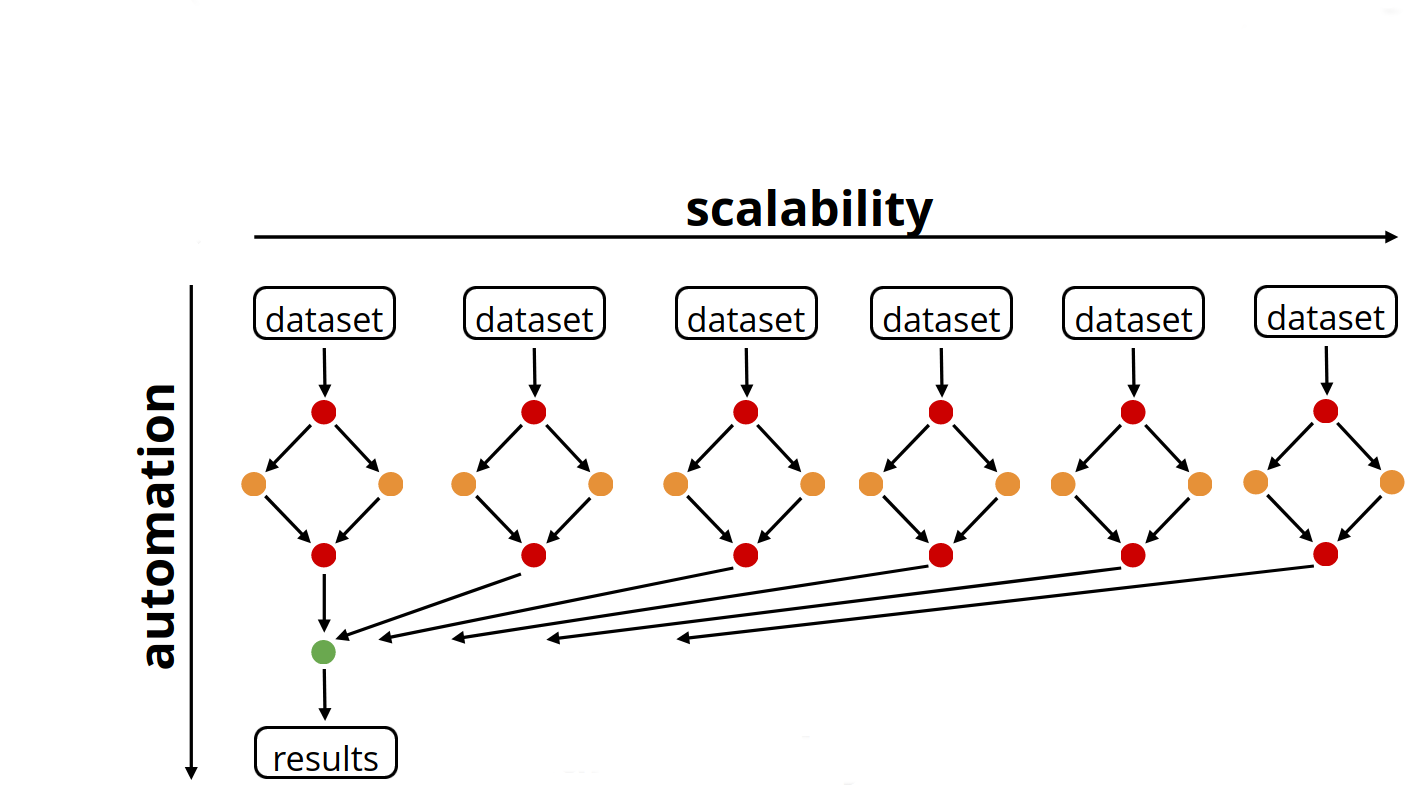
\includegraphics[width=0.7\textwidth]{Snakemake/scalability.png}};
      \node at (8, 2.5) {\begin{minipage}{0.65\textwidth}
                             \textbf{Handle parallelization:}
                             \begin{itemize}
                                \item execute for tens of thousands of datasets
                                \item efficiently use any computing platform
                              \end{itemize}
                           \end{minipage}
                           };
    \end{tikzpicture}
  \end{onlyenv}
  \begin{onlyenv}<3| handout:1>
    \begin{tikzpicture}
      \path[use as bounding box] (0.7,0) rectangle (12,8);
      \node at (5.5, 5.5) {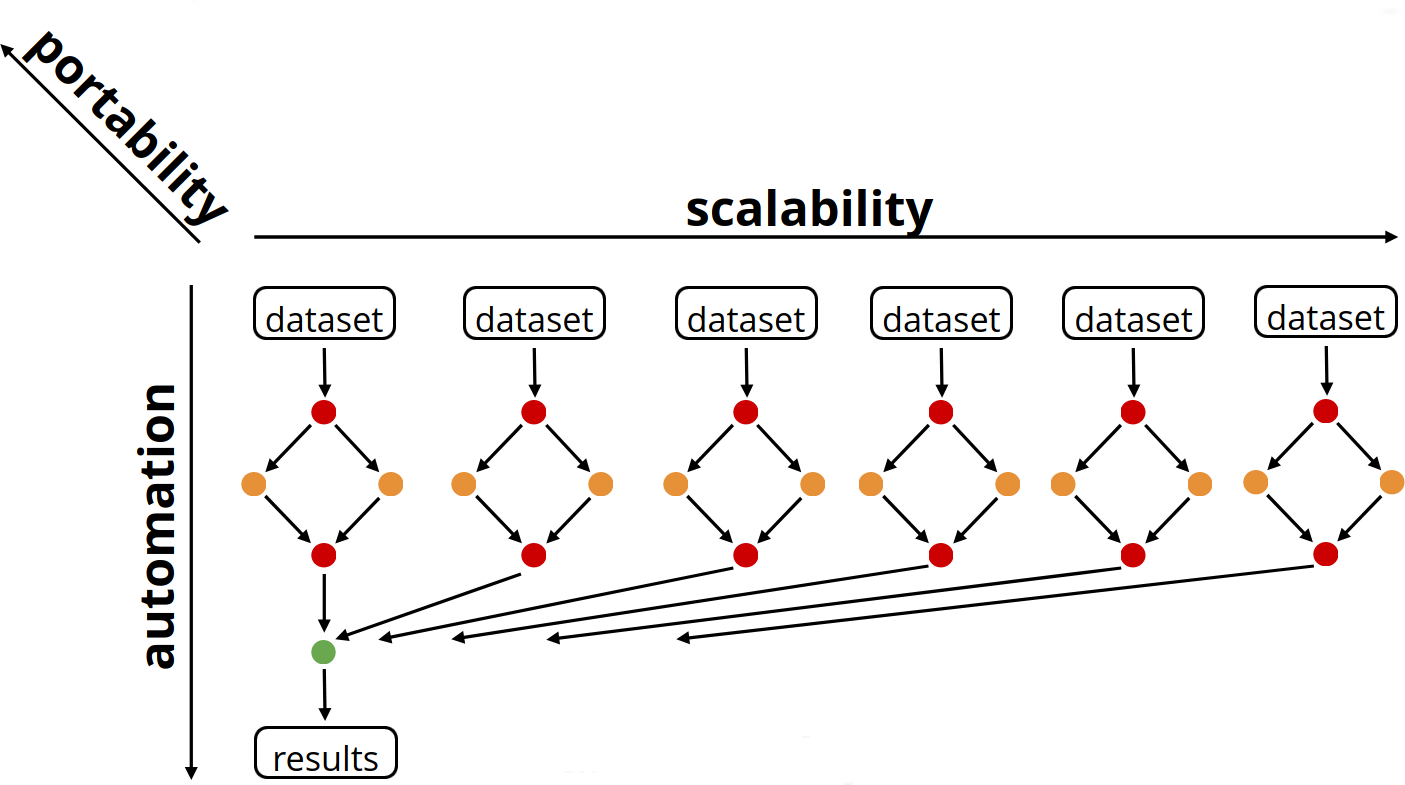
\includegraphics[width=0.7\textwidth]{Snakemake/portability.png}};
      \node at (8, 2.5) {\begin{minipage}{0.65\textwidth}
                             \textbf{Handle deployment:}\newline
                             be able to easily execute analyses on a different system/platform/infrastructure
                           \end{minipage}
                           };
    \end{tikzpicture}
  \end{onlyenv}
\end{frame}

%%%%%%%%%%%%%%%%%%%%%%%%%%%%%%%%%%%%%%%%%%%%%%%%%%%%%%%%%%%%%%%%%%%%%%%%%%%%%%%%
\begin{frame}
  \frametitle{Beyond Reproducibility}
  \begin{onlyenv}<1| handout:0>
    \begin{figure}
      \centering
      
\includegraphics[width=0.85\textwidth]{Snakemake/reproducibility_only.png}
    \end{figure}
  \end{onlyenv}
  \begin{onlyenv}<2| handout:0>
    \begin{figure}
      \centering
      
\includegraphics[width=0.85\textwidth]{Snakemake/reproducibility_empty.png}
    \end{figure}
  \end{onlyenv}
  \begin{onlyenv}<3| handout:0>
    \begin{figure}
      \centering
      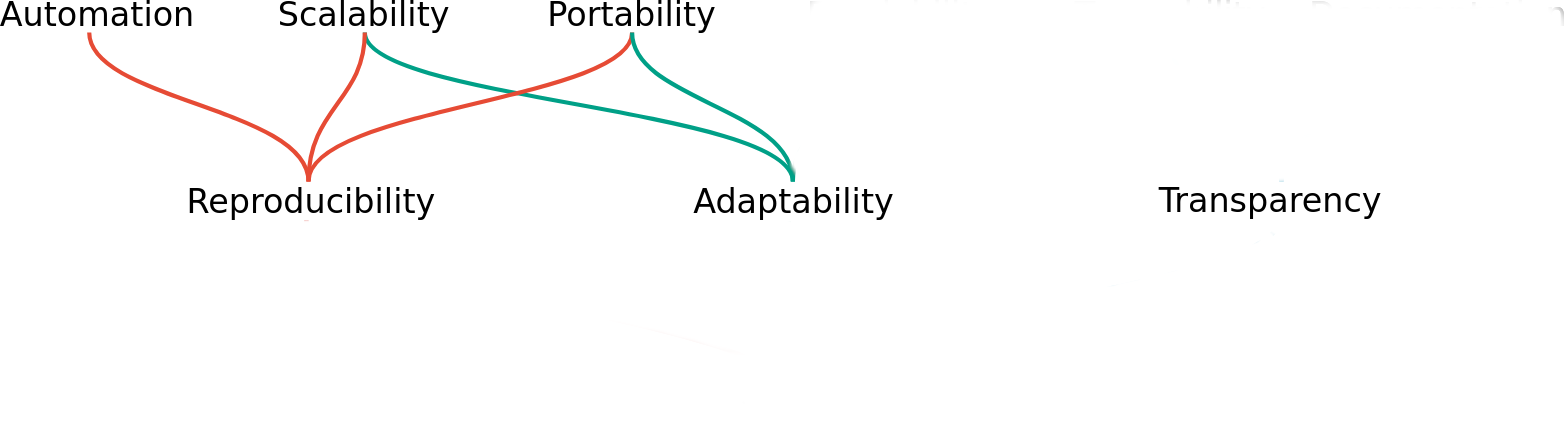
\includegraphics[width=0.85\textwidth]{Snakemake/reproducibility_left.png}
    \end{figure}
  \end{onlyenv}
    \begin{onlyenv}<4| handout:1>
      \begin{figure}
        \centering
        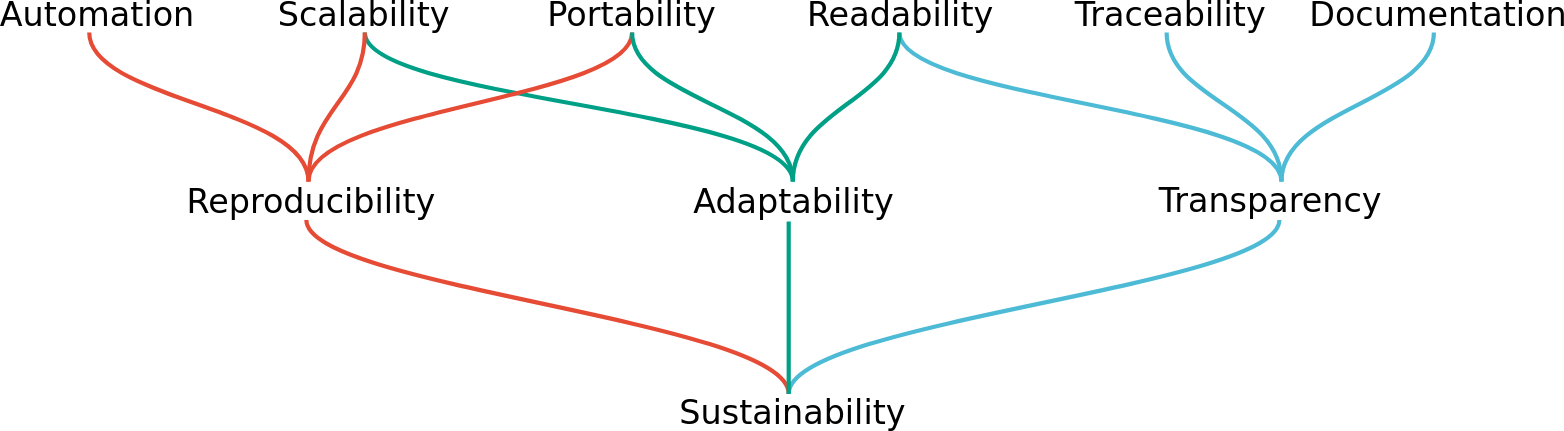
\includegraphics[width=0.85\textwidth]{Snakemake/reproducibility_full.png}
      \end{figure}
  \end{onlyenv}
\end{frame}

%%%%%%%%%%%%%%%%%%%%%%%%%%%%%%%%%%%%%%%%%%%%%%%%%%%%%%%%%%%%%%%%%%%%%%%%%%%%%%%%
\begin{frame}
  \frametitle{\Snakemake}
  \begin{figure}
    \centering
    \caption{\textbf{>370k} downloads since 2015\newline
             \textbf{>1300} citations\newline
             \textbf{>7} citations per week since 2021}
    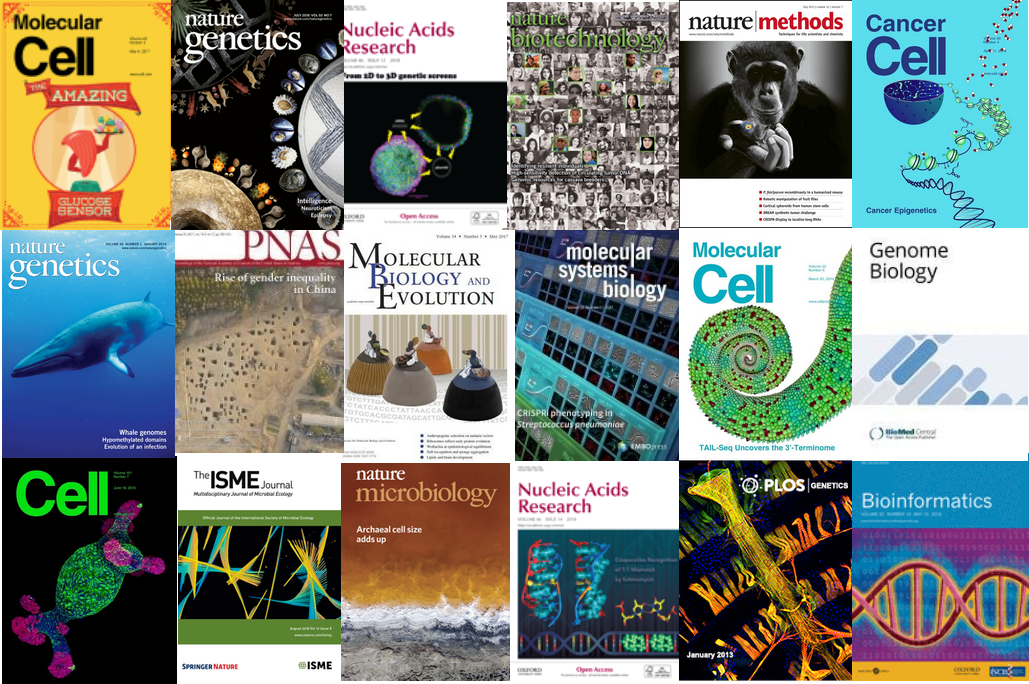
\includegraphics[width=0.6\textwidth]{Snakemake/paper_wall.png}
  \end{figure}
\end{frame}

%%%%%%%%%%%%%%%%%%%%%%%%%%%%%%%%%%%%%%%%%%%%%%%%%%%%%%%%%%%%%%%%%%%%%%%%%%%%%%%%
\begin{frame}
  \frametitle{The \Snakemake{} Catalogue}
  \begin{columns}
    \begin{column}{0.5\textwidth}
      \begin{itemize}[<+->]
   \item Extremely feature rich: \lhref{https://snakemake.github.io/snakemake-workflow-catalog/}{over 1800 workflows}
   \item Almost a hundred standardized workflows ready to use (meaning: well documented and with automatic deployment)
   \item Cluster batch systems are supported (and support for various cloud systems, too)
   \item There is an option to include Nextflow wrappers, too.
      \end{itemize}
    \end{column}
    \begin{column}{0.5\textwidth}
      \begin{figure}
        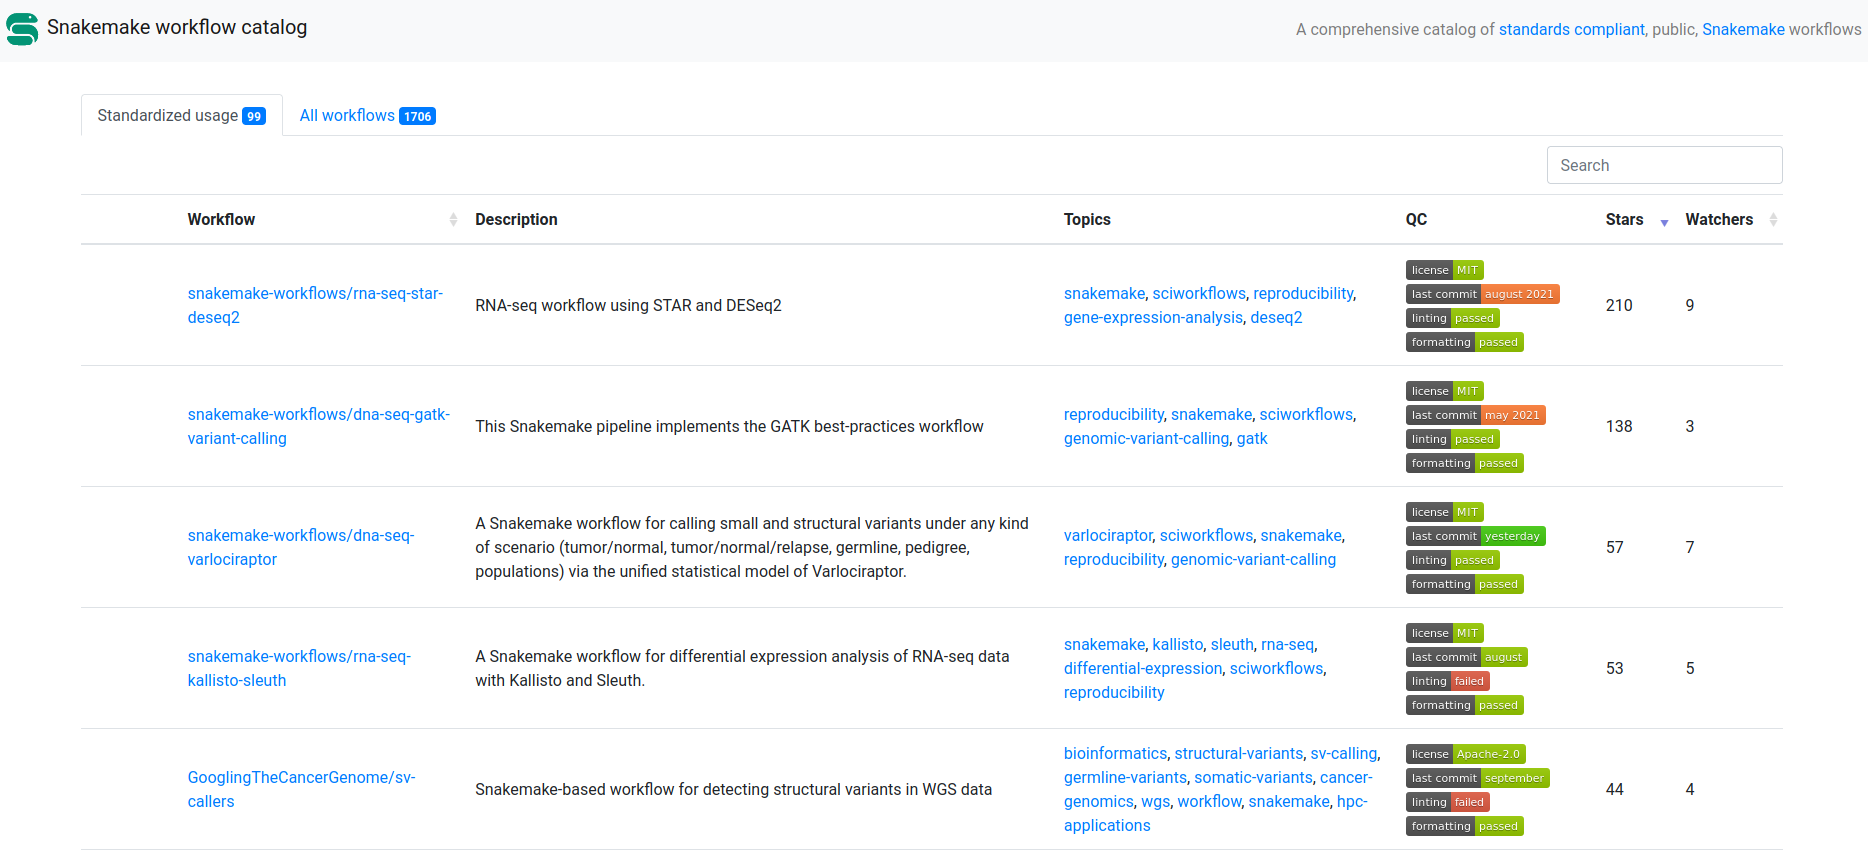
\includegraphics[width=\textwidth]{Snakemake/Snakemake_Workflow_Catalog.png}
        \caption{Screenshot of the Workflow Catalogue}
      \end{figure}
    \end{column}
  \end{columns}
\end{frame}


%%%%%%%%%%%%%%%%%%%%%%%%%%%%%%%%%%%%%%%%%%%%%%%%%%%%%%%%%%%%%%%%%%%%%%%%%%%%%%%%
\subsection{Goals, Background \& Outline}

%%%%%%%%%%%%%%%%%%%%%%%%%%%%%%%%%%%%%%%%%%%%%%%%%%%%%%%%%%%%%%%%%%%%%%%%%%%%%%%%
\begin{frame}
  \frametitle{Questions}
  \begin{question}[The questions you most probably have when starting your Analysis:]
  	\begin{itemize}
      \item How to start quickly (with the lowest amount of overhead)?
      \item What are the necessary tools?
    \end{itemize}
  \end{question}
                                                                               
  \begin{question}[Our question to you:]
  	 How do you get this information? And: Is reproducibility and sustainability your concern?
  \end{question}
  \pause
  \begin{block}{Most frequent Sources}
   \begin{itemize}
    \item Your labmate(s)
    \item The Internet
    \item Yes, of course ... eventually, when I brag about my paper/thesis.
   \end{itemize}
  \end{block}
\end{frame}

%%%%%%%%%%%%%%%%%%%%%%%%%%%%%%%%%%%%%%%%%%%%%%%%%%%%%%%%%%%%%%%%%%%%%%%%%%%%%%%%
\begin{frame}
  \frametitle{The Workflow Approach}
  Workflow Engines answer these questions directly by providing
  \begin{itemize}
   \item entire Workflows can be selected and can be put to action.
   \item executing routines reliably.
  \end{itemize}
\end{frame}

%%%%%%%%%%%%%%%%%%%%%%%%%%%%%%%%%%%%%%%%%%%%%%%%%%%%%%%%%%%%%%%%%%%%%%%%%%%%%%%%
\begin{frame}
  \frametitle{Going HPC}
  \begin{question}
  	Why would you want to work on a cluster?
  \end{question}
  \pause
  Answers may include:
  \begin{itemize}[<+->]
   \item compute power and ressources for big data
   \item launching scalable (and otherwise portable) workflows with workflow engines
  \end{itemize}
\end{frame}
